\begin{dang}{Thực tế}
    \begin{itemize}
        \item \textbf{Giả thiết có sẵn hàm số $y=f(x)$:} áp dụng cách giải dạng toán tìm Max-min của hàm một biến để tìm $x$ rồi kết luận.
        \item \textbf{Tự xây dựng nên hàm số $y=f(x)$:} sử dụng các kiến thức về hình học, vật lý để tìm ra hàm $f(x)$, một số mối quan hệ thường dùng là: $v=s'$, $a=v'=s''$.
    \end{itemize}
\end{dang}
\begin{vd}
    Trong một thí nghiệm y học, người ta cấy $1\,000$ vi khuẩn vào môi trường dinh dưỡng. Bằng thực nghiệm, người ta xác định được số lượng vi khuẩn thay đổi theo thời gian bởi công thức: $$N(t)=1\,000+\dfrac{100t}{100+t^2}\text{ (con),}$$ trong đó $t$ là thời gian tính bằng giây (\textit{Nguồn: R. Larson and B. Edwards, Calculus 10e, Cengage 2014}). Tính số lượng vi khuẩn lớn nhất kể từ khi thực hiện cấy vi khuẩn vào môi trường dinh dưỡng.
    \loigiai{
        \noindent Xét hàm số $N(t)=1\,000+\dfrac{100t}{100+t^2}\ (t>0)$.\\
        Ta có $N'(t)=\dfrac{100\cdot(100+t^2)-100\cdot2t}{\left(100+t^2\right)^2}=\dfrac{100\cdot\left(100-t^2\right)}{\left(100+t^2\right)^2}$.\\
        Cho $N'(t)=0 \Leftrightarrow 100-t^2=0 \Leftrightarrow \hoac{&t=10&&(\text{thoả } t>0)\\ &t=-10.&&(\text{không thoả } t>0)}$\\
        Bảng biến thiên
        \begin{center}
            
\begin{tikzpicture}[thick,font=\footnotesize]
                \tikzset{double style/.append style={double distance=1.5pt}}
                \tkzTabInit[lgt=1.5,espcl=2.5,deltacl=.75,color,colorL=green!60!yellow!50,colorV=green!60!yellow!50,lw=.35pt]
                {$t$/0.8,$N'(t)$/0.8,$N(t)$/2.5}
                {$0$,$10$,$+\infty$}
                \tkzTabLine{,+,0,-,}
                \tkzTabVar{-/$1\,000$,+/$1\,005$,-/$1\,000$}
            \end{tikzpicture}
        \end{center}
        Căn cứ vào bảng biến thiên, ta thấy: Trên khoảng $(0;+\infty)$ hàm số $N(t)$ đạt giá trị lớn nhất bằng $1\,005$ tại $x=10$.\\
        Vậy số vi khuẩn lớn nhất kể từ khi thực hiện cấy vi khuẩn vào môi trường dinh dưỡng là $1\,005$ con.
    }
\end{vd}
\begin{vd}%[KSCL T12, Chu Văn An, Hà Nội, 2018]%[Trần Bá Huy, 12EX-9-2018]%[2D1K3-6]%
    Một chất điểm chuyển động theo quy luật $s(t)=t^2-\dfrac{1}{6}t^3$ (m). Tìm thời điểm $t$ (giây) mà tại đó vận tốc $v$ (m/s) của chuyển động đạt giá trị lớn nhất.
    % \choice
    % {\True $t=2$}
    % {$t=0{,}5$}
    % {$t=2{,}5$}
    % {$t=1$}
    \loigiai{
        Ta có $v(t)=s'(t)=2t-\dfrac{1}{2}t^2$. Suy ra $v'(t)=2-t$ và $v'(t)=0\Leftrightarrow t=2$.\\
        Bảng biến thiên
        \begin{center}
            
\begin{tikzpicture}[>=stealth]
                \tkzTabInit[lgt=1.2,espcl=2]
                {$t$ /0.8, $v'(t)$ /0.8, $v(t)$ /2}
                {$ $, $2$, $ $}
                \tkzTabLine{ , +, 0, -, }
                \tkzTabVar{-/, +/ $2$, -/}
            \end{tikzpicture}
        \end{center}
        Vậy chất điểm đạt vận tốc lớn nhất tại thời điểm $t=2$ (giây).
    }
\end{vd}
\begin{vd}%[2D1K3-6]%Ví dụ 3:
    Một người muốn làm một bồn chứa $1\,000$ lít hình trụ có nắp đậy. Tìm chiều cao $h$ (dm) của bồn để ít tốn vật liệu nhất.
    \begin{center}
        \begin{tikzpicture}[scale=0.7, font=\footnotesize, line join=round, line cap=round, >=stealth]
            \def \x{2} %bán kính trục lớn elip
            \def \y{0.8} %bán kính trục bé elip
            \def \h{3} %chiều cao hình trụ
            \coordinate (A) at (0,0);
            \coordinate (B) at (2*\x,0);
            \coordinate (O) at ($(A)!0.5!(B)$);
            \coordinate (O') at ($(O)+(0,\h)$);
            \coordinate (A') at ($(A)+(0,\h)$);
            \coordinate (B') at ($(B)+(0,\h)$);
            \draw[dashed] (B) arc(0:180:\x cm and \y cm);
            \draw (B) arc(0:-180:\x cm and \y cm);
            \draw (O') ellipse (\x cm and \y cm);
            \tkzDrawSegments(A,A' B,B');
            \draw[<->] (2*\x+0.7,0)--(2*\x+0.7,\h);
            \node at (2*\x+0.7,0.5*\h) [right]{$h$};
        \end{tikzpicture}
    \end{center}
    \loigiai{
        Để ít tốn vật liệu nhất thì diện tích toàn phần bồn nước phải nhỏ nhất.\\
        Tức là $S_{tp}=2\pi R^2+2\pi Rh$ nhỏ nhất (với $R$ là bán kính đường tròn đáy).\\
        Thể tích bồn nước $V=\pi R^2h=1000\Rightarrow R=\sqrt{\dfrac{1000}{\pi h}}$.\\
        Khi đó $S_{tp}=2\pi\cdot\dfrac{1000}{\pi h}+2\pi\sqrt{\dfrac{1000}{\pi h}}h=\dfrac{2000}{h}+\sqrt{4000\pi h}$.\\
        $\Rightarrow S'_{tp}=-\dfrac{2000}{h^2}+\dfrac{2000\pi}{\sqrt{4000\pi h}}, S'_{tp}=0\Leftrightarrow\sqrt{4000\pi h}=\pi h^2\Leftrightarrow h=\sqrt[3]{\dfrac{4000}{\pi}}$.\\
        Sử dụng bảng biến thiên, ta tìm được $S_{tp}$ nhỏ nhất khi $h=\sqrt[3]{\dfrac{4000}{\pi}}$.
    }
\end{vd}
\BTTN
\Opensolutionfile{ans}[ans/2D1-3-DANG-3]
\begin{ex}%[2D1B3-6]%[Dự án TEX hóa đề cương Marie Curie - Ân Trương]
    Một chất điểm chuyển động theo phương trình $
    s(t)=-\dfrac{21}{6} t^{3}+\dfrac{2017}{4} t^{2}+t-\dfrac{110}{23}$ trong đó $ t $ tính bằng giây và $ s $ tính bằng mét. Thời điểm vận tốc của chất điểm đạt giá trị lớn nhất gần với con số nào sau đây ?
    \choice
    {$28,7s$}
    {$33,6s$}
    {\True$48s$}
    {$72,1s$}
    \loigiai{
        Ta có $
        s(t)=-\dfrac{21}{6} t^{3}+\dfrac{2017}{4} t^{2}+t-\dfrac{110}{23} \Rightarrow v(t)=s'(t)=-\dfrac{21}{2}t^2+\dfrac{2017}{2}t+1$.\\
        Ta có $ v'(t)=-21t+\dfrac{2017}{2} $.\\
        Cho $ v'(t)=0 \Leftrightarrow t=\dfrac{2017}{42}$.
        Ta có bảng biến thiên của hàm số $ y=v(t) $
        \begin{center}
            
\begin{tikzpicture}
                \tkzTabInit[nocadre=false,lgt=1.2,espcl=2.5,deltacl=1]
                {$t$ /1,$v’(t)$ /1,$v(t)$ /2.5}
                {$0$,$\dfrac{2017}{42}$,$+\infty$}
                \tkzTabLine{,+,0,-,}
                \tkzTabVar{-/,+/$v\left (\dfrac{42}{2017}\right )$,-/}
            \end{tikzpicture}
        \end{center}
        Dựa vào bảng biến thiên, $ \max\limits_{[0 ;+\infty)}v(t)=v\left (\dfrac{2017}{42}\right ) $.\\
        Vậy vận tốc của chất điểm đạt giá trị lớn nhất khi $ t=\dfrac{2017}{42} \approx 48s $.
    }
\end{ex}
%Cau 65
\begin{ex}%[2D1B3-6]%[Dự án TEX hóa đề cương Marie Curie - Ân Trương]
    Một chất điểm chuyển đông theo phương trình $ s(t)=-t^3+9t^2+t+10 $ trong đó $ t $ tính bằng giây và $ s $ tính bằng mét. Thời điểm vận tốc của chất điểm đạt giá trị lớn nhất là
    \choice
    {$t=5s$}
    {$t=6s$}
    {$t=2s$}
    {\True$t=3s$}
    \loigiai{
        Ta có $
        s(t)=s(t)=-t^3+9t^2+t+10 \Rightarrow v(t)=s'(t)=-3t^2+18t+1$.\\
        Ta có $ v'(t)=-6t+18$.\\
        Cho $ v'(t)=0 \Leftrightarrow t=3$.
        Ta có bảng biến thiên của hàm số $ y=v(t) $
        \begin{center}
            
\begin{tikzpicture}
                \tkzTabInit[nocadre=false,lgt=1.2,espcl=2.5,deltacl=0.6]
                {$t$ /0.6,$v’(t)$ /0.6,$v(t)$ /2}
                {$0$,$3$,$+\infty$}
                \tkzTabLine{,+,0,-,}
                \tkzTabVar{-/,+/$v\left (3\right )$,-/}
            \end{tikzpicture}
        \end{center}
        Dựa vào bảng biến thiên, $ \max\limits_{[0 ;+\infty)}v(t)=v\left (3\right ) $.\\
        Vậy thời điểm vận tốc của chất điểm đạt giá trị lớn nhất tại $ t=3s $
    }
\end{ex}
%Câu 66
\begin{ex}%[2D1B3-6]%[Dự án TEX hóa đề cương Marie Curie - Ân Trương]
    Một vật chuyển động theo quy luật $ s(t)=-\dfrac{1}{3}t^3+6t^2 $ với $ t $ (giây) là khoảng thời giai từ khi vật bắt đầu chuyển động và $ s $ (mét) là quãng đường vật di chuyển trong thời gian đó. Hỏi trong khoảng thời gian $ 9$ giây, kể từ lúc bắt đầu chuyển động, vận tốc lớn nhất vật đạt được bằng bao nhiêu ?
    \choice
    {\True$36 m/s$}
    {$243 m/s$}
    {$27 m/s$}
    {$144 m/s$}
    \loigiai{
        Ta có $s(t)=-\dfrac{1}{3}t^3+6t^2 \Rightarrow v(t)=s'(t)=-t^2+12t$.\\
        Do ta cần tìm $ v_{\max}(t) $ trong $ 9 $ giây đầu tiên nên ta cần tìm giá trị lớn nhất của hàm số $ y=v(t)=-t^2+12t $ trên $ [0;9] $. \\
        Ta có $ v'(t)=-2t+12 $.\\
        Cho $ v'(t)=0 \Leftrightarrow t=6 $.\\
        Ta có $ v(0)=0 $, $ v(6)=36 $, $ v(9)=27$ nên $ \max\limits_{[0 ; 9]}v(t)=v(6)=36 $.\\
        Vậy vận tốc lớn nhất vật đạt được bằng $ 36 $ m/s.
    }
\end{ex}
%Câu 67
\begin{ex}%[2D1B3-6]%[Dự án TEX hóa đề cương Marie Curie - Ân Trương]
    Một vật chuyển động theo quy luật $ s(t)=-\dfrac{1}{2}t^3+9t^2 $ với $ t $ (giây) là khoảng thời giai từ khi vật bắt đầu chuyển động và $ s $ (mét) là quãng đường vật di chuyển trong thời gian đó. Hỏi trong khoảng thời gian $ 10 $ giây, kể từ lúc bắt đầu chuyển động, vận tốc lớn nhất vật đạt được bằng bao nhiêu ?
    \choice
    {$216 $ m/s}
    {$30 $ m/s}
    {$64 $ m/s}
    {\True$54 $ m/s}
    \loigiai{
        Ta có $s(t)=-\dfrac{1}{2}t^3+9t^2 \Rightarrow v(t)=s'(t)=-\dfrac{3}{2}t^2+18t$.\\
        Do ta cần tìm $ v_{\max}(t) $ trong $ 10 $ giây đầu tiên nên ta cần tìm giá trị lớn nhất của hàm số $ y=v(t)=-\dfrac{3}{2}t^2+18t $ trên $ [0;10] $. \\
        Ta có $ v'(t)=-3t+18 $.\\
        Cho $ v'(t)=0 \Leftrightarrow t=6 $.\\
        Ta có $ v(0)=0 $, $ v(6)=54 $, $ v(10)=30$ nên $ \max\limits_{[0 ; 10]}v(t)=v(6)=54$.\\
        Vậy vận tốc lớn nhất vật đạt được bằng $ 54 $ m/s.
    }
\end{ex}
\begin{ex}%Ví dụ 15%[Phat Dang Tan - DA1]%[2D1B3-6]
    Cho một tấm nhôm hình vuông cạnh $12$ cm. Người ta cắt ở bốn góc của tấm nhôm đó bốn hình vuông bằng nhau, mỗi hình vuông có cạnh bằng $x$ cm, rồi gập tấm nhôm lại như hình vẽ dưới đây để được một cái hộp không nắp. Tìm giá trị của $x$ để hộp nhận được có thể tích lớn nhất.
    \begin{center}
        \begin{tikzpicture}[scale=0.8, font=\footnotesize, >=stealth]
            \coordinate (A) at (0,0);
            \coordinate (B) at (4,0);
            \coordinate (C) at (4,4);
            \coordinate (D) at (0,4);
            \draw (A) -- (B) -- (C) -- (D) -- (A);
        \end{tikzpicture}
        \hspace{1cm}
        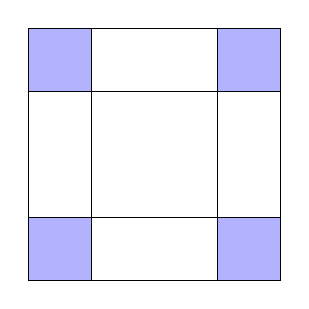
\begin{tikzpicture}[scale=0.8, font=\footnotesize, >=stealth]
            \coordinate (A) at (0,0);
            \coordinate (B) at (4,0);
            \coordinate (C) at (4,4);
            \coordinate (D) at (0,4);
            \fill[blue!30](A)--(1,0)--(1,1)--(0,1)--cycle;
            \fill[blue!30](B)--(3,0)--(3,1)--(4,1)--cycle;
            \fill[blue!30](C)--(3,4)--(3,3)--(4,3)--cycle;
            \fill[blue!30](D)--(1,4)--(1,3)--(0,3)--cycle;
            \draw (A) -- (B) -- (C) -- (D) -- (A);
            \draw (1,0) -- (1,4) (3,0) -- (3,4) (0,1) -- (4,1) (0,3) -- (4,3);
        \end{tikzpicture}
        \hspace{1cm}
        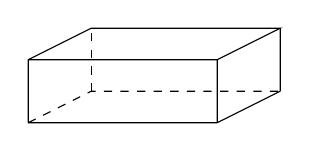
\begin{tikzpicture}[scale=0.8, font=\footnotesize, >=stealth]
            \coordinate (A) at (0,0);
            \coordinate (B) at (3,0);
            \coordinate (C) at (4,0.5);
            \coordinate (D) at (1,0.5);
            \coordinate (E) at (0,1);
            \coordinate (F) at (3,1);
            \coordinate (G) at (4,1.5);
            \coordinate (H) at (1,1.5);
            \draw (A) -- (B)--(C) (A)--(E) (B)--(F) (C)--(G);
            \draw (E) -- (F) -- (G) -- (H) -- (E);
            \draw[dashed] (A)--(D)--(C);
            \draw[dashed] (D)--(H);
        \end{tikzpicture}
    \end{center}
    \choice
    {$(-\infty; 0)$}
    {$(-\infty;+\infty)$}
    {\True $(0;+\infty)$}
    {$(-1; 1)$}
    \loigiai{
        Ta có $V(x)=(12-2x)^2\cdot x=4x^3-48x^2+144x$\quad $\left(0<x<6\right)$.\\
        $V'(x)=12x^2-96x+144=0\Leftrightarrow \hoac{&x=6 \text{ (loại) }\\&x=2 \text{ (nhận).}}$\\
        Bảng biến thiên
        \begin{center}
            
\begin{tikzpicture}
                \tkzTabInit[nocadre=false,lgt=1.2,espcl=2.5,deltacl=0.6]
                {$x$ /0.6,$f'(x)$ /0.6,$f(x)$ /2}
                {$0$,$2$,$6$}
                \tkzTabLine{,+,$0$,-,}
                \tkzTabVar{-/$0$, +/$128$,-/$0$}
            \end{tikzpicture}
        \end{center}
        Suy ra $\max\limits_{(0;6)} V=128$ khi $x=2$.\\
        Vậy khối hộp có thể tích lớn nhất là $128 \text{ cm}^3$ khi $x=2$ cm.
    }
\end{ex}
\begin{ex}%Ví dụ 16%[Phat Dang Tan - DA1]%[2D1B3-6]
    \immini{Cho một tấm tôn hình chữ nhật có kích thước	$80$ cm x $50$ cm. Người ta cắt bốn góc của tấm nhôm đó bốn hình vuông bằng nhau, mỗi hình có cạnh $x$ cm để khi gập lại được một	chiếc hộp không nắp. Để chiếc hộp có thể tích lớn nhất thì giá trị của $x$ bằng bao nhiêu?
        \choice
        {$(-\infty; 0)$}
        {$(-\infty;+\infty)$}
        {\True $(0;+\infty)$}
        {$(-1; 1)$}}
    {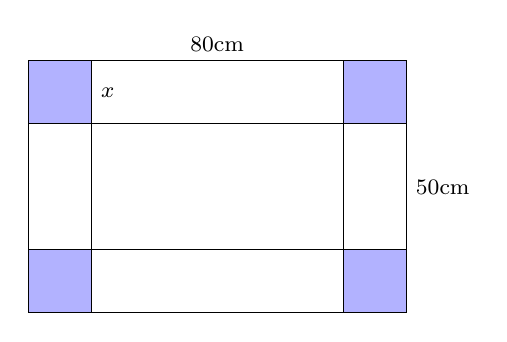
\begin{tikzpicture}[scale=0.8, font=\footnotesize, >=stealth]
            \coordinate (A) at (0,0);
            \coordinate (B) at (6,0);
            \coordinate (C) at (6,4);
            \coordinate (D) at (0,4);
            \fill[blue!30](A)--(1,0)--(1,1)--(0,1)--cycle;
            \fill[blue!30](B)--(5,0)--(5,1)--(6,1)--cycle;
            \fill[blue!30](C)--(5,4)--(5,3)--(6,3)--cycle;
            \fill[blue!30](D)--(1,4)--(1,3)--(0,3)--cycle;
            \draw (A) -- (B) -- (C) -- (D) -- (A);
            \draw (1,0) -- (1,4) (5,0) -- (5,4) (0,1) -- (6,1) (0,3) -- (6,3);
            \coordinate[label=above:{$80$cm}] (c) at (3,4);
            \coordinate[label=right:{$50$cm}] (b) at (6,2);
            \coordinate[label=right:{$x$}] (d) at (1,3.5);
    \end{tikzpicture}}
    \loigiai{
        Ta có $V=(80-2x)\cdot(50-21)\cdot x=4x^3-260x^2+4000x$\quad $\left(0<x<25\right)$.\\
        $V'(x)=12x^2-520x+4000=0\Leftrightarrow \hoac{&x=\dfrac{100}{3} \text{ (loại) }\\&x=10 \text{ (nhận).}}$\\
        Bảng biến thiên
        \begin{center}
            
\begin{tikzpicture}
                \tkzTabInit[nocadre=false,lgt=1.2,espcl=2.5,deltacl=0.6]
                {$x$ /0.6,$f'(x)$ /0.6,$f(x)$ /2}
                {$0$,$10$,$25$}
                \tkzTabLine{,+,$0$,-,}
                \tkzTabVar{-/$0$, +/$18000$,-/$0$}
            \end{tikzpicture}
        \end{center}
        Suy ra $\max\limits_{(0;25)} V=18000$ khi $x=10$.\\
        Vậy chiếc hộp có thể tích lớn nhất là $18000 \text{ cm}^3$ khi $x=10$ cm.
    }
\end{ex}
\begin{ex}%[2D1K3-6]%
    \immini{Tính diện tích lớn nhất $S_{\max}$ của một hình chữ nhật nội tiếp trong nửa đường tròn bán kính $R=6 \;\mathrm{cm}$ nếu một cạnh của hình chữ nhật nằm dọc theo đường kính của hình tròn mà hình chữ nhật đó nội tiếp.}
    {\begin{tikzpicture}[scale=.8, line join=round, line cap=round,>=stealth]
            \tikzset{label style/.style={font=\footnotesize}}
            \draw[name path=v] (3,0) arc (0:180:3cm);
            \coordinate (M) at (-3,0);
            \coordinate (N) at (3,0);
            \draw[name path=MN] (M)--(N);
            \coordinate (O) at (0,0);
            \coordinate (C) at (2,0);
            \coordinate (D) at (-2,0);
            \coordinate (A) at (-2,2.236);
            \coordinate (B) at (2,2.236);
            \tkzDrawSegments(A,B B,C C,D D,A)
            \tkzDrawPoints[fill=black,size=2pt](A,B,C,D)
            \tkzFillPolygon[pattern=north east lines](A,B,C,D)
    \end{tikzpicture}}
    \choice
    {$S_{\max} =36\pi \;\mathrm{cm}^2$}
    {\True $S_{\max} =36 \;\mathrm{cm}^2$}
    {$S_{\max} =96\pi \;\mathrm{cm}^2$}
    {$S_{\max} =18 \;\mathrm{cm}^2$}
    \loigiai{
        \immini{Gọi hình chữ nhật cần tính diện tích là $ABCD$ có $OC=x (0<x<6)$, $OB=6$.\\
            Khi đó diện tích của hình chữ nhật $ABCD$ là $S=AB\cdot BC =2x\sqrt{36-x^2} =f(x)$.}
        {\begin{tikzpicture}[scale=.8, line join=round, line cap=round,>=stealth]
                \tikzset{label style/.style={font=\footnotesize}}
                \draw[name path=v] (3,0) arc (0:180:3 cm);
                \coordinate (M) at (-3,0);
                \coordinate (N) at (3,0);
                \draw[name path=MN] (M)--(N);
                \coordinate (O) at (0,0);
                \coordinate (C) at (2,0);
                \coordinate (D) at (-2,0);
                \coordinate (A) at (-2,2.236);
                \coordinate (B) at (2,2.236);
                \tkzDrawSegments(A,B B,C C,D D,A)
                \tkzDrawPoints[fill=black,size=2pt](A,B,C,D,O)
                \coordinate (x) at ($(O)!0.5!(C)$);
                \tkzLabelPoints[below](O,C,D,x)
                \tkzLabelPoints[above left](A)
                \tkzLabelPoints[above right](B)
                \tkzFillPolygon[pattern=north east lines](A,B,C,D)
        \end{tikzpicture}}
        \noindent Diện tích lớn nhất của hình chữ nhật $ABCD$ là giá trị lớn nhất của $f(x) =2x\sqrt{36-x^2}$ trên $(0; 6)$.\\
        $f'(x)=2\sqrt{36-x^2}-\dfrac{2x^2}{\sqrt{36-x^2}} =\dfrac{-4x^2+72}{\sqrt{36-x^2}}$.\\
        $f'(x)=0\Leftrightarrow\hoac{&x=3\sqrt{2}\in(0; 6)\\&x=-3\sqrt{2}\notin(0; 6).}$ \\
        $BBT$
        \begin{center}
            
\begin{tikzpicture}[scale=.9]
                \tkzTabInit[espcl=2.5,lgt=1.5,nocadre]
                {$x$/0.7,$f'(x)$/0.7,$f(x)$/1.7}
                {$0$,$3\sqrt 2$,$6$}
                \tkzTabLine{,+,0,-,}
                \tkzTabVar{-/$0$,+/$36$,-/$0$}
            \end{tikzpicture}
        \end{center}
        Ta có: $\max\limits_{(0; 6)} f(x)=36$.\\
        Vậy $S_{\max} =36 \;\mathrm{cm}^2$.}
\end{ex}
%\begin{ex}%[GHK2, Bắc Yên Thành Nghệ An, 2018]%[Bùi Thanh Cương 12EX-5, Lê Thị Thúy Hằng 12EX-5(ID6)]%[2D1K3-6]%
% \immini{Một tấm kẽm hình vuông $ABCD$ có cạnh bằng $30$ cm. Người ta gập tấm kẽm theo hai cạnh $EF$ và $GH$ cho đến khi cạnh $AD$ và $BC$ trùng nhau như hình vẽ bên để được một hình lăng trụ khuyết hai đáy. Giá trị của $x$ để thể tích khối lăng trụ lớn nhất là
% \choice
% {$x=5$ cm}
% {$x=9$ cm}
% {$x=8$ cm}
% {\True $x=10$ cm}
% }{%Hình ảnh bên phải
% \begin{tikzpicture}[scale=0.8,line join= around, line cap= around,>=stealth]
% \tkzDefPoint[label=90:$A$](1,6){A}
% \tkzDefPoint[label=90:$B$](8,6){B}
% \tkzDefPoint[label=-60:$C$](8,1){C}
% \tkzDefPoint[label=-120:$D$](1,1){D}
% \tkzDefPoint[label=90:$E$](3,6){E}
% \tkzDefPoint[label=-60:$F$](3,1){F}
% \tkzDefPoint[label=-120:$H$](6,1){H}
% \tkzDefPoint[label=90:$G$](6,6){G}
% \draw[<->] (1,0.5) -- (3,0.5);\node at (2,0.7) {$x$};
% \draw[<->] (6,0.5) -- (8,0.5);\node at (7,0.7) {$x$};
% \draw[<->] (1,0) -- (8,0);\node at (5,-0.3) {$30$ cm};
% \tkzDefPoint[label=90:$G$](13,6){Q1}
% \tkzDefPoint[label=90:$E$](10,6){M1}
% \tkzDefPoint[label=-90:$F$](10,1){N1}
% \tkzDefPoint[label=-90:$H$](13,1){P1}
% \tkzDefPoint[label=-90:$D \equiv C$](11.5,0){A1}
% \tkzDefPoint[label=-90:$A\equiv B$](11.5,5){B1}
% \tkzDrawPoints[fill=black](A,B,C,D,E,F,G,H,N1,P1,M1,Q1,A1,B1)
% \tkzDrawSegments(A,B B,C C,D D,A E,F G,H N1,A1 A1,P1 P1,Q1 Q1,M1 M1,B1 B1,Q1 B1,A1 M1,N1)
% \tkzDrawSegment[dashed](N1,P1)
% \end{tikzpicture}
% }
% \loigiai{
% Do chiều cao cố định nên khối lăng trụ có thể tích lớn nhất khi diện tích đáy lớn nhất. Vì đáy là tam giác cân với cạnh bên bằng $x$ nên ta tính được diện tích \\
% $$S=\dfrac{1}{2}(30-2x).\sqrt{x^2-\dfrac{(30-2x)^2}{4}}=(15-x)\sqrt{30x-225} \,\, \text{với} \,\, x \in (0,15).$$
% $S'=-\sqrt{30x-225}+(15-x)\dfrac{15}{\sqrt{30x-225}}$.
% \begin{eqnarray*}
% & S'=0 & \Leftrightarrow \dfrac{15}{\sqrt{30x-225}}=\sqrt{30x-225}+(15-x) \\
% & & \Leftrightarrow \heva{& 30x -225 >0\\ & 45x=450} \\
% & & \Leftrightarrow\heva{& x> \dfrac{15}{2}\\ & x=10} \\
% & & \Leftrightarrow x=10.
% \end{eqnarray*}
% }
%\end{ex}
\begin{ex}%[Đề HK1, SGDDT Quảng Trị 2017]%[Phan Hoàng Anh 12-EX-5]%[2D1K3-6]%
    Một tấm tôn hình chữ nhật có kích thước $80\mathrm{cm}\times50\mathrm{cm}$, người ta cắt ở bốn góc của tấm tôn đó bốn hình vuông bằng nhau, mỗi hình vuông có cạnh bằng $x$(cm) rồi gập tấm tôn lại để được một cái thùng hình hộp chữ nhật không nắp. Tìm $x$ để thùng có thể tích lớn nhất.
    \choice
    {$ x=8 $}
    {\True $ x=10 $}
    {$ x=9 $}
    {$ x=11 $}
    \loigiai{sau khi cắt bỏ bốn góc và gập tấm tôn lại, ta thu được một hình hộp chữ nhật với kích thước đáy là $(80-2x)\mathrm{cm}\times(50-2x)\mathrm{cm}$, chiều cao là $x$.\\
        Thể tích của thùng là $V=(80-2x)(50-2x)x=4x^3-260x^2+4000x=f(x)$.\\
        \immini{$f'(x)=12x^2-520x+4000$, $f'(x)=0\Leftrightarrow\hoac{&x=10\\&x=\dfrac{100}{3}}$.\\
            Do $ 0<x<25 $ nên nhận $x=10$.\\
            Dựa vào bảng biến thiên ta suy ra thể tích thùng lớn nhất khi $x=10$.}
        {
\begin{tikzpicture}
                \tkzTabInit[lgt=1.6,espcl=1.8,nocadre]
                {$x$/0.7,$y'$/0.7,$y$/1.8}{$0$,$10$,$25$}
                \tkzTabLine{,+,0,-,}
                \tkzTabVar{-/$ $,+/$ $,-/$ $}
    \end{tikzpicture}}}
\end{ex}
\begin{ex}%[Đề kiểm tra HKI Toán 12 - Năm học 2017 - 2018 - Chuyên Amsterdam Hà Nội]%[Lê Đức Việt, dự án EX5-2018]%[2D1K3-6]%
    \immini{Một bác thợ muốn chế một chiếc thùng đựng nước hình trụ, mặt xung quanh của thùng được cuộn từ những mặt tôn hình chữ nhật có chu vi $4{,}8$ m. Hỏi bác thợ phải chọn những tấm tôn có kích thước như thế nào để chiếc thùng đựng được nhiều nước nhất?}
    {
        \begin{tikzpicture}[scale=0.18, line join=round, line cap=round,>=stealth]
            \draw (-30,0)--(-10,0)--(-10,10)--(-30,10)--(-30,0);
            \draw (5,0)--(5,10) (-5,10)--(-5,0);
            \draw[black] (5,0)arc(0:-180:5 and 1.6);
            \draw[dashed] (5,0)arc(0:180:5 and 1.6);
            \draw[black] (5,10)arc(0:360:5 and 1.6);
        \end{tikzpicture}
    }
    \choice
    { $1{,}2$m và $1{,}2$m}
    {\True$1{,}6$m và $0{,}8$m}
    {$1{,}8$m và $0{,}6$m}
    {$1{,}4$m và $1{,}0$m}
    \loigiai{ Gọi $x$ mét là $1$ kích thước của tấm tôn hình chữ nhật (ĐK: $0<x<2{,}4$). \\ Suy ra $2{,}4-x$ là kích thước còn lại của tấm tôn.\\ Giả sử cuộn tấm tôn với bán kính của đường tròn đáy là $\dfrac{2{,}4-x}{2\pi}$ mét.
        \\
        Suy ra thể tích chiếc thùng đựng nước là: $V=\pi \left(\dfrac{2{,}4-x}{2\pi}\right)^2x=\dfrac{x^3-4{,}8x^2+5{,}76x}{4\pi} \\ \Rightarrow V'=\dfrac{3x^2-9{,}8x+5{,}76}{4\pi}$.\\ Cho $V'=0$ (PTVN), Suy ra hàm $V$ đồng biến trên khoảng $(0; 2{,}4)$, nên V không đạt giá trị lớn nhất.\\
        Vậy thùng nước phải được cuốn với bán kính của đường tròn đáy là $\dfrac{x}{2\pi}$.\\
        Suy ra thể tích chiếc thùng đựng nước là $V=\pi \dfrac{x^2}{(4\pi)^2}(2{,}4-x)=\dfrac{-x^3+2{,}4x^2}{4\pi} \\ \Rightarrow V'=\dfrac{-3x^2+4{,}8x}{4\pi}$.\\ Cho $V'=0 \Leftrightarrow \hoac{x&=0\\x&=1{,}6}$. So với điều kiện suy ra $x=1{,}6$. \\ Vậy kích thước của tấm tôn để tạo ra chiếc thùng có thể đựng nhiều nước nhất là $1{,}6$ mét và $0{,}8$ mét.
    }
\end{ex}
\begin{ex}%[Thi HK1, THPT Nguyễn Thị Minh Khai HCM, 2020]%[Sơn Bùi, 12EX-HK1-HCM]%[2D1K3-6]%
    Một toán công nhân cần xây một hố ga không nắp có dạng hình hộp chữ nhật với thể tích $3,2$ m$^3$, chiều cao của hố ga gấp đôi chiều rộng của đáy hố ga. Hãy xác định diện tích của đáy hố ga để khi xây tiết kiệm nguyên vật liệu nhất?
    \choice
    {$16$ m$^2$}
    {\True $1,6$ m$^2$}
    {$1,2$ m$^2$}
    {$12$ m$^2$}
    \loigiai{Gọi $x$ là chiều rộng hố ga thì $2x$ là chiều cao hố ga. Gọi $y$ là chiều dài hố ga ($x,y>0$, đơn vị: m).\\
        Theo đề bài, ta có $2x^2y=3,2\Rightarrow y=\dfrac{1{,}6}{x^2}$.\\
        Diện tích xây hố ga chính là bốn mặt xung quanh và một mặt đáy, tức là $$S=2\left(x\cdot 2x+\dfrac{1,6}{x^2}\cdot 2x\right)+x\cdot\dfrac{1{;}6}{x^2}=4x^2+\dfrac{8}{x}$$
        Theo bất đẳng thức Cô-si cho 3 số dương ta có
        $$S=4x^2+\dfrac{4}{x}+\dfrac{4}{x}\ge 3\sqrt[3]{4x^2\cdot \dfrac{4}{x}\cdot \dfrac{4}{x}}=12.$$
        Đẳng thức xảy ra khi $4x^2=\dfrac{4}{x}\Leftrightarrow x=1$.\\
        Khi đó diện tích đáy hố ga là $x\cdot \dfrac{1,6}{x^2}=1{,}6$ m$^2$.}
\end{ex}
\begin{ex}%[GHKII, THPT Chuyên Quốc Học Huế, năm 2020 - 2021]%[Nguyễn Tài Tuệ, 12EX6]%[2D1K3-6]%
    Một sợi dây kim loại dài $120 \mathrm{~cm}$ được cắt thành hai đoạn. Đoạn dây thứ nhất được uốn thành hình vuông, đoạn dây thứ hai được uốn thành vòng tròn (tham khảo hình bên dưới).
    \begin{center}
        \begin{tikzpicture}[scale=1, font=\footnotesize, line join=round, line cap=round, >=stealth]
            \path
            (0,0) coordinate (A)
            (8,0) coordinate (B)
            (3,0) coordinate (M)
            (1.5,-3) coordinate (C)
            (4.5,-2) coordinate (D)
            ;
            \draw (A)--(B);
            \draw (C) circle (1cm);
            \draw (D) rectangle (6.5,-4);
            \tkzDrawPoints[fill=black](A,B,M)
            \draw[->,dashed] (A) arc (180:226:3);
            \draw[->,dashed] (M) arc (0:-46:3);
            \draw[->,dashed] (M) arc (180:240:3);
            \draw[->,dashed] (B) arc (0:-60:3);
            \draw (4,0) node[above]{$ 120 $ cm};
            % \draw (A) node[above]{$ A $} (M) node[above]{$ C $};
        \end{tikzpicture}
    \end{center}
    \noindent
    Tổng diện tích của hình vuông và hình tròn đạt giá trị nhỏ nhất là (làm tròn đến hàng đơn vị)
    \choice
    {\True $504$}
    {$498$}
    {$462$}
    {$426$}
    \loigiai{
        \begin{center}
            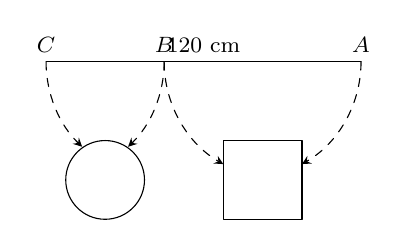
\begin{tikzpicture}[scale=0.5, font=\footnotesize, line join=round, line cap=round, >=stealth]
                \path
                (0,0) coordinate (A)
                (8,0) coordinate (B)
                (3,0) coordinate (M)
                (1.5,-3) coordinate (C)
                (4.5,-2) coordinate (D)
                ;
                \draw (A)--(B);
                \draw (C) circle (1cm);
                \draw (D) rectangle (6.5,-4);
                \tkzDrawPoints[fill=black](A,B,M)
                \draw[->,dashed] (A) arc (180:226:3);
                \draw[->,dashed] (M) arc (0:-46:3);
                \draw[->,dashed] (M) arc (180:240:3);
                \draw[->,dashed] (B) arc (0:-60:3);
                \draw (4,0) node[above]{$ 120 $ cm};
                \draw (A) node[above]{$ C $} (M) node[above]{$ B $} (B)node[above]{$ A $};
            \end{tikzpicture}
        \end{center}
        Đặt $A B=x \Rightarrow B C=120-x(0<x<120)$.\\
        Chu vi của đường tròn là $2 \pi r=120-x \Rightarrow r=\dfrac{120-x}{2 \pi}$.\\
        Diên tích hình tròn là $S_{\text{đt}}=\pi r^2=\dfrac{(120-x)^2}{4\pi}$.\\
        Diện tich hình vuông $S_{\text{hv}}=\left(\dfrac{x}{4}\right)^2=\dfrac{x^2}{16}$.\\
        Tồng diện tich của hình vuông và hình tròn là $S=\dfrac{(120-x)^2}{4\pi}+\dfrac{x^2}{16}=f(x)$.\\
        Xét $f(x)=\dfrac{(120-x)^2}{4\pi}+\dfrac{x^2}{16}$ trên $ (0;120) $ ta có\\
        $f'(x)=\dfrac{(4+\pi)x-480}{8\pi};f'(x)=0 \Leftrightarrow (4+\pi)x-480=0 \Leftrightarrow x=\dfrac{480}{4+\pi}$.\\
        Bảng biến thiên
        \begin{center}
            
\begin{tikzpicture}[scale=1, font=\footnotesize, line join=round, line cap=round, >=stealth]
                \tkzTabInit[nocadre=false,lgt=1.2,espcl=2.5,deltacl=0.6]
                {$x$ /0.6,$f’(x)$ /0.6,$f(x)$ /2}
                {$0$,$\tfrac{480}{4+\pi}$,$120$}
                \tkzTabLine{ ,-,z,+, }
                \tkzTabVar{+/,-/$504{,}1$,+/}
            \end{tikzpicture}
        \end{center}
        Vây $S_{\min }=\min\limits _{(0.120)} f(x) \approx 504$.
    }
\end{ex}
\BTTL
\begin{ex}%[TeX hóa SGK CTST 12]%[Nguyen Huynh]%[2D1H3-6]
    Khi làm nhà kho, bác An muốn cửa sổ có dạng hình chữ nhật với chu vi bằng $4 \mathrm{~m}$ (Hình 6). Tìm kích thước khung cửa sổ sao cho diện tích cửa sổ lớn nhất (để hứng được nhiều ánh sáng nhất)?
    \shortans{}
    \loigiai{
        Gọi chiều dài của khung cửa sổ là $x$ (mét). Điều kiện $0<x<2$.\\
        Suy ra chiều rộng của khung cửa sổ là $2-x$ (mét).\\
        Khi đó diện tích của khung cửa sổ là $x\left(2-x\right)=-x^2+2x$.\\
        Đặt $f(x)=-x^2+2x\Rightarrow f'(x)=-2x+2=0\Leftrightarrow x=1$. Ta có bảng biến thiên như sau
        \begin{center}
            
\begin{tikzpicture}[font=\normalsize,t style/.style={style=solid}]
                %dòng khai báo
                \tkzTabInit[lgt=1.2,espcl=2.5,deltacl=0.5]
                {$x$ /0.75, $f'(x)$/0.75, $f(x)$/2}
                {$ 0$,$ 1 $,$ 2$}
                %dòng xét dấu
                \tkzTabLine{ , +,0 , -, } % z, t, d;
                %dòng biến thiên
                \tkzTabVar{-/$0$,+/$1$,-/$0$} %+ hoac-
            \end{tikzpicture}
        \end{center}
        Như bảng biến thiên ta thấy được diện tích khung của sổ lớn nhất khi $x=1$ hay khung cửa có dạng hình vuông cạnh $1$ mét.}
\end{ex}
\begin{ex}%[TeX hóa SGK CTST 12]%[Nguyen Huynh]%[2D1H3-6]
    Khối lượng $q$ (kg) của một mặt hàng mà cửa tiệm bán được trong một ngày phụ thuộc vào giá bán $p$ (nghìn đồng/kg) theo công thức $p=15-\dfrac{1}{2} q$. Doanh thu từ việc bán mặt hàng trên của cửa tiệm được tính theo công thức $R=p q$.
    \begin{enumerate}
        \item Viết công thức biểu diễn $R$ theo $p$.
        \item Tìm giá bán mỗi kilôgam sản phẩm để đạt được doanh thu cao nhất và xác định doanh thu cao nhất đó.
    \end{enumerate}
    \shortans{}
    \loigiai{
        \begin{enumerate}
            \item Ta có $p=15-\dfrac{1}{2} q$ $\Rightarrow q=30-2p$.\\
            Lại có $R=pq=p\left(30-2p\right)\Rightarrow R=-2p^2+30p$ với $0<p$.
            \item Xét $R'=-4p+30=0\Leftrightarrow p=7{,}5$.
            Ta có bảng biến thiên như sau
            \begin{center}
                
\begin{tikzpicture}[font=\normalsize,t style/.style={style=solid}]
                    %dòng khai báo
                    \tkzTabInit[lgt=1,espcl=2.5,deltacl=0.6]
                    {$x$ /0.75, $R'$/0.75, $R$/2}
                    {$ 0$,$ 7{,}5 $,$ +\infty$}
                    %dòng xét dấu
                    \tkzTabLine{ , +,0 , -, } % z, t, d;
                    %dòng biến thiên
                    \tkzTabVar{-/$0$,+/$112{,}5$,-/$-\infty$} %+ hoac-
                \end{tikzpicture}
            \end{center}
            Từ bảng biến thiên thấy để đạt được doanh thu cao nhất thì giá bán mỗi kilôgam sản phẩm $p=7{,}5$ (nghìn đồng/kg) khi đó doanh thu cao nhất sẽ là $R(7{,}5)=112{,}5$ (nghìn đồng).
    \end{enumerate}}
\end{ex}
\begin{ex}%[TeX hóa SGK CTST 12]%[Nguyen Huynh]%[2D1H3-6]
    Hộp sữa $1$ lít được thiết kế dạng hình hộp chữ nhật với đáy là hình vuông cạnh $x$ cm. Tìm $x$ để diện tích toàn phần của hộp nhỏ nhất.
    \shortans{}
    \loigiai{
        Thể tích hộp sữa là $1\ \mathrm{l}=1\ \mathrm{dm}^3=1000\ \mathrm{cm}^3$ khi đó chiều cao của hộp sữa là $\dfrac{1000}{x^2}$ (cm).\\
        Đặt diện tích toàn phần của hộp sữa là $y=2x^2+4x\cdot \dfrac{1000}{x^2}=\dfrac{2x^3+4000}{x}$ (cm)$^2$.\\
        Xét $y'=\dfrac{4x^3-4000}{x^2}=0\Leftrightarrow x=10$ (cm).\\
        Ta có bảng biến thiên như sau
        \begin{center}
            
\begin{tikzpicture}[font=\normalsize,t style/.style={style=solid}]
                %dòng khai báo
                \tkzTabInit[lgt=1,espcl=2.65,deltacl=0.6]
                {$x$ /0.75, $y'$/0.75, $y$/2}
                {$ 0$,$ 10 $,$ +\infty$}
                %dòng xét dấu
                \tkzTabLine{ , -,0 , +, } % z, t, d;
                %dòng biến thiên
                \tkzTabVar{+/$+\infty$,-/$600$,+/$+\infty$} %+ hoac-
            \end{tikzpicture}
        \end{center}
        Vậy theo bảng biến thiên ta thấy $x=10$ (cm) thì diện tích toàn phần của hộp sữa sẽ nhỏ nhất là $600\ {\rm cm^2}$. }
\end{ex}
\begin{ex}
    Trong $5$ giây đầu tiên, một chất điểm chuyển động theo phương trình $$s(t)=-t^3+6t^2+t+5,$$ trong đó $t$ tính bằng giây và $s$ tính bằng mét. Chất điểm có vận tốc tức thời lớn nhất bằng bao nhiêu trong $5$ giây đầu tiên đó?
    \shortans{}
    \loigiai{
        \noindent Xét hàm số $s(t)=-t^3+6t^2+t+5$, trên đoạn $\left[0;5\right]$.\\
        Đạo hàm $s'(t)=-3t^2+12t+1.$\\
        Cho $s'(t)=0 \Leftrightarrow -3t^2+12t+1=0 \Leftrightarrow \hoac{&x=\dfrac{6+\sqrt{39}}{3}\in[0;5]\\&x=\dfrac{6-\sqrt{39}}{3}\notin[0;5].}$\\
        Các giá trị $f(0)=5$, $f\left(\tfrac{6+\sqrt{39}}{3}\right)\approx41{,}04$, $f(5)=35$.\\
        So sánh các giá trị, ta có $\max\limits_{[0;5]}f(x)\approx41{,}04$, $\min\limits_{[0;5]}f(x)=5$.
    }
\end{ex}
%----------Bài 6
\begin{ex}
    Người ta bơm xăng vào bình xăng của một xe ô tô. Biết rằng thể tích $V$ (lít) của lượng xăng trong bình xăng tính theo thời gian bơm xăng $t$ (phút) được cho bởi công thức $$V(t)=300(t^2-t^3)+4 \text{ với } 0\le t\le 0{,}5.$$
    \begin{flushright}
        \textit{(Nguồn: R.I. Charles et al., Algebra 2, Pearson)}
    \end{flushright}
    \begin{enumerate}[a)]
        \item Ban đầu trong bình xăng có bao nhiêu lít xăng?
        \item Sau khi bơm $30$ giây thì bình xăng đầy. Hỏi dung tích của bình xăng trong xe là bao nhiêu lít?
        \item Khi xăng chảy vào bình xăng, gọi $V(t)$ là tốc độ tăng thể tích tại thời điểm $t$ với $0\le t\le 0{,}5$. Xăng chảy vào bình xăng ở thời điểm nào có tốc độ tăng thể tích là lớn nhất?
    \end{enumerate}
    \shortans{}
    \loigiai{
        \begin{enumerate}[a)]
            \item Số xăng trong bình ban đầu là $V(0)=4$ lít.
            \item Dung tích bình xăng $V=V\left(\dfrac{1}{2}\right)=41{,}5$ lít.
            \item Xét hàm số $V(t)=300(t^2-t^3)+4 \text{ với } 0\le t\le 0{,}5.$\\
            Đạo hàm $V'(t)=300t(2-3t)$.\\
            Cho $V'(t)=0 \Leftrightarrow 300t(t-3t)=0 \Leftrightarrow \hoac{&t=0\in[0;0{,}5]\\&t=\dfrac{2}{3}\notin[0;0{,5}].}$\\
            Các giá trị $V(0)=4$, $V\left(\dfrac{1}{2}\right)=41{,}5$.\\
            Xăng chảy vào bình xăng vào thời điểm ở giây thứ $30$ có tốc độ tăng thể tích là lớn nhất.
        \end{enumerate}
    }
\end{ex}
%----------Bài 7
\begin{ex}
    Ho ép khí quản lại, ảnh hưởng đến tốc độ của không khí đi vào khí quản. Tốc độ của không khí đi vào khí quản khi ho được cho bởi công thức $$V=k(R-r)r^2 \text{ với } 0\le r<R,$$ trong đó $k$ là hằng số, $R$ là bán kính bình thường của khí quản, $r$ là bán kính khí quản kho ho (\textit{Nguồn: R. Lason and B. Edwards, Calculus 10e, Cengage 2014}). Hỏi bán kính của khí quản khi ho bằng bao nhiêu thì tốc độ của không khí đi vào khí quản là lớn nhất?
    \shortans{}
    \loigiai{
        \noindent
        Xét hàm số $V=k(R-r)r^2$ trên nửa khoảng $[0;R)$\\
        Ta có $V(r)=k(R-r)r^2 \Rightarrow V'(r)=-3kr^2+2kRr=-kr(3r-2R)$.\\
        Cho $V'(r)=0 \Leftrightarrow -kr(3r-2R)=0 \Leftrightarrow \hoac{&r=0&\in[0;R)\\&r=\dfrac{2R}{3}&\in[0;R)}$.\\
        Các giá trị $V(0)=0$, $V\left(\dfrac{2R}{3}\right)=4k\left(\dfrac{R}{3}\right)^3$.\\
        Bán kính khí quản lớn nhất khi $r=\dfrac{2R}{3}$.\\
        Bảng biến thiên\\
        \begin{tikzpicture}[thick,font=\footnotesize, >=stealth]
            \tkzTabInit[lgt=1.25,espcl=2.25,deltacl=.35,lw=.5pt,color,colorL=violet!25!,colorV=violet!25!]
            {$r$/1.2,$V'(r)$/0.8,$V(r)$/3.5}
            {$-\infty$,$0$,$\dfrac{2R}{3}$,$R$,$+\infty$}
            \tkzTabLine{,-,0,+,0,-,,-}
            \draw (N12) node[below](A){$+\infty$}
            ($(N12)!1/2!(N33)$) node[](B){$0$}
            (N32) node[below](C){$\dfrac{4kR^3}{27}$}
            ($(N32)!1/2!(N53)$) node[xshift=-1mm](D){$0$}
            (N53) node[above](E){$-\infty$}	;
            \draw[->,orange] (A)--(B); \draw[->,orange] (B)--(C);
            \draw[->,orange] (C)--(E);
            \draw[pattern={Lines[angle=60,distance=1.25mm]},pattern color=blue,thin] (N11)--($(N21)+(180:1.25mm)$)--($(N23)+(180:1.25mm)$)--(N13);
            \draw[pattern={Lines[angle=120,distance=1.25mm]},pattern color=blue,thin] (N51)--(N41)--(N43)--(N53);
        \end{tikzpicture}
        Căn cứ vào bảng biến thiên, ta có $\max\limits_{[0;R)}V(r)=V\left(\dfrac{2R}{3}\right)=4k\left(\dfrac{R}{3}\right)^3=\dfrac{4kR^3}{27}$.
    }
\end{ex}
\begin{ex}
    \immini{Một thùng chứa nhiên liệu gồm phần ở giữa là một hình trụ có chiều dài $h$ mét $(h>0)$ và hai đầu là các nửa hình cầu bán kính $r$ $(r>0)$ (\textit{Hình 1.11}). Biết rằng thể tích của thùng chứa là $144\,000 \pi$ m$^3$. Để sơn mặt ngoài của phần hình cầu cần $20\,000$ đồng cho $1$ m$^2$, còn sơn mặt ngoài cho phần hình trụ cần $10\,000$ đồng cho $1$ m$^2$. Xác định $r$ để chi phí cho việc sơn diện tích mặt ngoài thùng chứa (bao gồm diện tích xung quanh hình trụ và diện tích hai nửa hình cầu) là nhỏ nhất, biết rằng bán kính $r$ không được vượt quá $50$ m.
    }{
        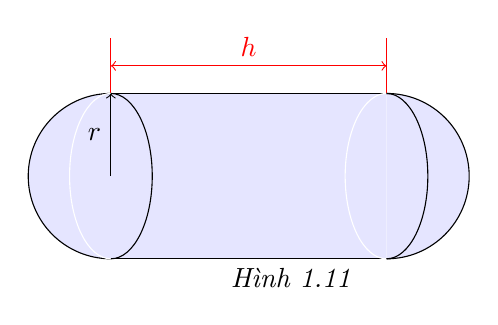
\begin{tikzpicture}[scale=.7]
            \draw[white,fill=blue!10] (0,0) rectangle (5,3);
            \draw(0,0)--(5,0);
            \draw(0,3)--(5,3);
            \draw[red](0,3)--(0,4);
            \draw[red](5,3)--(5,4);
            \draw[fill=blue!10] (5,3) arc(90:-90:1.5);
            \draw[fill=blue!10] (0,0) arc(-90:-270:1.5);
            \draw[white] (0,3) arc (90:270:0.75 and 1.5);
            \draw (0,0) arc (-90:90:0.75 and 1.5);
            \draw[white] (5,3) arc (90:270:0.75 and 1.5);
            \draw (5,0) arc (-90:90:0.75 and 1.5);
            \draw[red,<->] (0,3.5)--(5,3.5) node[midway,above]{$h$};
            \draw[->] (0,1.5)--(0,3) node[midway,left]{$r$};
            \draw (2,0) node[below right]{\textit{Hình 1.11}};
        \end{tikzpicture}
    }
    \shortans{}
    \loigiai{
        Ta có thể tích của thùng chứa nhiên liệu là $V=\pi \cdot r^2 \cdot h + \dfrac{4}{3} \pi \cdot r^3 = 144\, 000 \pi$ \\
        Suy ra $h=\dfrac{(144\,000-\dfrac{4}{3} \cdot r^3)}{r^2}$ \\
        Khi đó chi phí sơn diện tích mặt ngoài thùng chứa là
        $$2 \pi \cdot r \cdot \dfrac{(144\,000-\dfrac{4}{3} \cdot r^3)}{r^2} \cdot 10^4 + 4 \pi \cdot r^2 \cdot 2 \cdot 10^4 =2 \pi \cdot 10^4 \left( \dfrac{144\,000}{r} + \dfrac{8}{3} r^2 \right). $$
        Xét hàm số $f(r)=\dfrac{144\,000}{r} + \dfrac{8}{3} r^2$ với $r \in (0;50]$\\
        Ta có $f'(r)=-\dfrac{144\,000}{r^2} + \dfrac{16}{3} r=\dfrac{16r^3-432\,000}{3r^2}$ và $f'(r)=0 \Leftrightarrow r=30$ m.\\
        Bảng biến thiên\\
        \begin{center}
            
\begin{tikzpicture}
                \tkzTabInit[nocadre=false,lgt=1.2,espcl=3.5,deltacl=0.6]
                {$r$/1,$f'(r)$/1,$f(r)$/3}
                {$0$,	$30$,	$50$}
                \tkzTabLine{,	-,	$0$,	+}
                \tkzTabVar{+/$+\infty$,	-/$7200$,	+/$9546{,}7$}
            \end{tikzpicture}
        \end{center}
        Vậy với $r=30$ m thì chi phí cho việc sơn diện tích mặt ngoài của thùng chứa là nhỏ nhất.
    }
\end{ex}
\begin{ex}
    Một doanh nghiệp tư nhân $A$ chuyên kinh doanh xe gắn máy các loại. Hiện nay doanh nghiệp đang tập trung vào chiến lược kinh doanh xe $X$ với chi phí mua vào một chiếc là 27 triệu đồng và bán ra với giá 31 triệu đồng. Với giá bán này, số lượng xe mà khách hàng đã mua trong một năm là 600 chiếc. Nhằm mục tiêu đẩy mạnh hơn nữa lượng tiêu thụ dòng xe đang bán chạy này, doanh nghiệp dự định giảm giá bán. Bộ phận nghiên cứu thị trường ước tính rằng nếu giảm 1 triệu đồng mỗi chiếc xe thì số lượng xe bán ra trong một năm sẽ tăng thêm 200 chiếc. Hỏi theo đó, giá bán mới là bao nhiêu thì lợi nhuận thu được cao nhất?
    \shortans{}
    \loigiai{
        Gọi giá bán mới là $x$ (triệu đồng) với $x \in [27;31]$.\\
        Khi đó số xe bán ra là $600+(31-x) \cdot 200$.\\
        Lợi nhuận thu được là
        \begin{eqnarray*}
            f(x) &=& [600+(31-x) \cdot 200](x-27)\\
            &=& (-200x+6800)(x-27)\\
            &=& -200x^2+12200x-183600\\
            &=& -200\left(x-\dfrac{61}{2}\right)^2+2450\\
            &\leq&2450.
        \end{eqnarray*}
        Vậy giá bán mới là $30,5$ triệu đồng thì lợi nhuận thu được là lớn nhất là $2\,450$ (triệu đông).
    }
\end{ex}
\begin{ex}%[2D1T3-2]
    Một nhà sản xuất cần làm ra những chiếc bình có dạng hình trụ với dung tích $1000\mathrm{~cm}^3$. Mặt trên và mặt dưới của bình được làm bằng vật liệu có giá 1,2 nghìn đồng$/\mathrm{cm}^2$, trong khi mặt bên của bình được làm bằng vật liệu có giá $0{,}75$ nghìn đồng$/\mathrm{cm}^2$. Tìm các kích thước của bình để chi phí vật liệu sản xuất mỗi chiếc bình là nhỏ nhất.
    \shortans{}
    \loigiai{
        %%%==============BT_1==============%%%
        \begin{bt}
            Gọi bán kính đáy của bình là $x$ (cm), ($x > 0$).\\
            Chiều cao của bình là $\dfrac{1000}{\pi \cdot x^2}$ (cm).\\
            Chi phí để sản xuất một chiếc bình là
            \[
            T(x)=2\cdot1{,}2\cdot\pi \cdot x^2+0{,}75\cdot \dfrac{2000}{x}=2{,}4\pi \cdot x^2+\dfrac{1500}{x}~\text{(nghìn đồng)}.
            \]
            Để chi phí sản xuất mỗi chiếc bình là thấp nhất thì $T(x)$ là nhỏ nhất.\\
            $T'(x)=4,8\pi x-\dfrac{1500}{x^2}, T'(x)=0\Leftrightarrow x=\sqrt[3]{\dfrac{625}{2\pi}}$ (thỏa mãn).\\
            Bảng biến thiên:
            \begin{center}
                
\begin{tikzpicture}[scale=1, font=\footnotesize]
                    \tkzTabInit[nocadre=false, lgt=1.2, espcl=2, deltacl=0.6]
                    {$x$/0.8,$T'(x)$/0.6,$T(x)$/2}
                    {$0$,$\sqrt[3]{\frac{625}{2\pi}}$,$12$};
                    \tkzTabLine{,-,$0$,+,};
                    \tkzTabVar{+/$+\infty$,-/$T\left(\sqrt[3]{\frac{625}{2\pi}}\right)$,+/$T(12)$};
                \end{tikzpicture}
            \end{center}
            Để chi phí sản xuất mỗi chiếc bình là nhỏ nhất thì bán kính đáy của bình là $\sqrt[3]{\dfrac{625}{2\pi}}$ cm và chiều cao của bình là $\dfrac{1000}{\pi \cdot\left(\sqrt[3]{\dfrac{625}{2\pi}}\right)^2}$ cm.
        \end{bt}
    }
\end{ex}
\begin{ex}%[2D1V3-6]%[GV- Thái Văn Sang]%[Du-An-Ngan-Hang-Cau-Hoi-2024-K12]%13
    Một vật chuyển động theo quy luật $s=-\dfrac{1}{3} t^3 + 6 t^2$ với $t$ (giây) là khoảng thời gian tính từ khi vật bắt đầu chuyển động và $s$ (mét) là quãng đường vật di chuyển được trong khoảng thời gian đó. Hỏi trong khoảng thời gian 9 giây, kể từ khi bắt đầu chuyển động, vận tốc lớn nhất của vật đạt được bằng bao nhiêu m/s?
    \shortans{$36$ m/s}
    \loigiai{
        Vận tốc của vật được tính bởi $v(t)=-t^2+12t$.\\
        Ta có $v'(t)=-2t+12$. Phương trình $v'(t)=0$ có nghiệm $t=6$.
        Bảng biến thiên
        \begin{center}
            
\begin{tikzpicture}
                \tkzTabInit[nocadre=false,lgt=1,espcl=3]
                {$t$ /0.6, $v'$ /.6,$v$ /1.8}
                {$0$ ,$6$ ,$9$}
                \tkzTabLine{,+,0,-,}
                \tkzTabVar{ -/$0$,+/$36$,-/$27$}
            \end{tikzpicture}
        \end{center}
        Dựa vào bảng biến thiên ta có vận tốc lớn nhất của vật đạt được bằng $36$ m/s.
    }
\end{ex}
\begin{ex}%[Dự án Tex hóa SKG KNTT - Nguyễn Mạnh Trung Anh]%[2D1V2-7]
    Giả sử doanh số (tính bằng sản phẩm) của một sản phẩm mới (trong một năm nhất định) tuân theo quy luật logistic được mô hình hóa bằng hàm số \[f(t)=\dfrac{5000}{1+5e^{-t}},\, t\ge0,\]
    trong đó thời gian $t$ được tính bằng năm, kể từ khi phát hành sản phẩm mới. Khi đó đạo hàm $f'(t)$ biểu thị tốc độ bán hàng. Hỏi sau khi phát hành bao nhiêu năm thì tốc độ bán hàng là lớn nhất?
    \shortans{$1{,}6$ năm }
    \loigiai{
        Gọi $g(t)$ là hàm tốc độ bán hàng.\\
        Khi đó $g(t)=f'(t)=\dfrac{25\,000e^{-t}}{(1+5e^{-t})^2}$, $t\ge0$.\\
        Ta có $g'(t)=\dfrac{25\,000e^{-t}(1+5e^{-t})(5e^{-t}-1)}{(1+5e^{-t})^4}$; $g'(t)=0\Leftrightarrow t=-\ln {\dfrac{1}{5}}$.\\
        Bảng biến thiên hàm số
        \begin{center}
            
\begin{tikzpicture}
                \tkzTabInit[nocadre=false,lgt=1.3,espcl=2.5,deltacl=0.6]
                {$t$ /0.6, $y'$ /0.6, $y$ /2.5}
                {$0$, $-\ln {\frac{1}{5}}$, $+\infty$}
                \tkzTabLine{,+,0,-,}
                \tkzTabVar{-/ $694{,}4$,+/$1250$,-/$0$}
            \end{tikzpicture}
        \end{center}
        Hàm số đạt cực đại tại $t=-\ln {\dfrac{1}{5}}\approx1{,}6$.\\
        Vậy sau khi phát hành $1{,}6$ năm thì tốc độ bán hàng là lớn nhất.
    }
\end{ex}
\Closesolutionfile{ans}